\documentclass[12pt]{report}

\usepackage{geometry}
\geometry{ b4paper, total={220mm,320mm}, left=20mm, top=15mm }

\usepackage{mathtools}
\usepackage{graphicx}
\usepackage{listings}
\usepackage{tikz}

%\usepackage{libertine, lato}

\usepackage{amssymb}
\usepackage{enumitem}
\usepackage{amsmath}


\usepackage{fontspec}
%\usepackage{microtype}

\usepackage{polyglossia}

\usepackage{hyperref}
\hypersetup{
    colorlinks=true,
    linkcolor=blue,
    filecolor=magenta,      
    urlcolor=cyan,
    pdftitle={Overleaf Example},
    pdfpagemode=FullScreen,
}
\urlstyle{same}


\graphicspath{ {img} }

\setmainfont{Georgia}
\setsansfont{Lato}
\setmonofont{Corbel}


\usetikzlibrary{arrows.meta}

\renewcommand{\thesection}{\Roman{section}}
\renewcommand{\thesubsection}{\thesection.\Roman{subsection}}

\title{\textsf{Οδηγός εγκατάστασης: GRC \& USRP\\
    \large Τμήμα Ηλεκτρολόγων Μηχανικών \& Μηχανικών Υπολογιστών \\
    Πανεπιστήμιο Δυτικής Μακεδονίας
}}
\author{\textsf{Μάρκος Δελαπόρτας} \footnote{E-mail: ece01316@uowm.gr}}
\date{\textsf{Mάρτιος 2024}}

\begin{document}

    \maketitle

    \section*{\textsf{Εγκατάσταση GNU Radio}}
        \subsection*{\textsf{Προαπαιτούμενα}}
        \begin{itemize}
            \item Εγκατεστημένο λειτουργικό σύστημα Linux - σε πραγματικό hardware ή σε vm
            (Ιδανικά Ubuntu/Debian LTS)
        \end{itemize}

        \subsection*{\textsf{Αρχικά}}
            Εγκαθιστούμε το GNU Radio, προτιμάμε το ντόπιο πακέτο και όχι απομονωμένες μορφές (όπως snap).
            Σε Ubuntu/Debian ανοίξτε ένα τερματικό και γράψτε:
            \begin{lstlisting}[language=bash]
                $ sudo apt update
                $ sudo apt install gnuradio
            \end{lstlisting}

            Αν χρειάζεστε περισσότερες πληροφορίες όπως διαφορετικές μεθόδους εγκατάστασης, απευθυνθείτε
            στην αυθεντική \href{ https://github.com/gnuradio/gnuradio}{σελίδα} του GNU Radio στο GitHub.

            Για να εκκινήσετε το GNU Radio γράψτε σε ένα τερματικό:
            \begin{lstlisting}[language=bash]
                $ gnuradio-companion
            \end{lstlisting}

    \section*{\textsf{Εγκατάσταση του driver για το USRP}}

        Το Universal Software Radio Peripheral (USRP B200/B210) είναι ένα μεσαίου/υψηλού επιπέδου 
        Software Defined Radio που αναπτύχθηκε από την Ettus Research η οποία είναι μια εταιρεία της
        National Instruments που επικεντρώνεται στην ανάπτυξη εξαιρετικά ευέλικτων SDR.
        (\href{https://www.ettus.com/products/}{περισσότερες πληροφορίες}). 
        Θα χρησιμοποιήσουμε το USRP B200 / B210 για τις εργαστηριακές συνεδρίες.

        \subsection*{\textsf{Εγκατάσταση του Προγράμματος Οδήγησης}}
            Βεβαιωθείτε ότι έχετε κλείσει το gnuradio (GRC). Ανοίξτε ένα τερματικό στον υπολογιστή
            Linux και εκτελέστε τις ακόλουθες εντολές:
            \begin{lstlisting}[language=bash]
                $ sudo add-apt-repository ppa:ettusresearch/uhd
                $ sudo apt update
                $ sudo apt install libuhd-dev uhd-host
            \end{lstlisting}
            Συνδέστε ένα USRP στον υπολογιστή σας και εκτελέστε την εντολή "uhd_find_devices" σε ένα τερματικό.
            \subsection*{\textsf{Έλεγχος Έκδοσης UHD}}
            Για να ελέγξετε εάν το πρόγραμμα οδήγησης έχει εγκατασταθεί σωστά:
            \begin{lstlisting}[language=bash]
                $ apt search "libuhd"
            \end{lstlisting}

        \subsection*{\textsf{είδωλα FPGA}}
            Αν το μπλοκ UHD (source/sink) στο GNU Radio δεν μπορεί να βρει τις εικόνες FPGA, βεβαιωθείτε
            ότι έχετε ελέγξει αν ο κατάλογος /usr/share/uhd/images/ υπάρχει και αν είναι κενός ή όχι.
            Βεβαιωθείτε ότι τα δυαδικά αρχεία usrp b200 fpga.bin και usrp b210 fpga.bin υπάρχουν σε 
            αυτόν το φάκελο. Ένα από αυτά τα αρχεία μεταφορτώνεται στο FPGA στο USRP κατά την εκτέλεση
            ενός διαγράμματος ροής GRC που περιέχει source ή/και sink USRP.

            Αν αυτός ο φάκελος δεν υπάρχει ή είναι κενός, εκτελέστε:
            \begin{lstlisting}[language=bash]
                $ sudo uhd_images_downloader
            \end{lstlisting}
            ή
            \begin{lstlisting}[language=bash]
                $ cd /usr/lib/uhd/utils/
                $ python3 uhd_images_downloader.py
            \end{lstlisting}

    \section*{\textsf{SDR Hello World}}
        \subsection*{Έλεγχος SDR}
            Για να λειτουργήσει οποιοδήποτε SDR στο GRC, πρέπει να βεβαιωθούμε ότι μπορούμε να
            "μιλήσουμε" στη συσκευή. Τα περισσότερα SDR είναι εξοπλισμένα με ένα εργαλείο λογισμικού
            για να ελέγξουν εάν η επικοινωνία με το υλικό λειτουργεί. Για τη συσκευή USRP αυτό 
            μπορεί να ελεγχθεί σε ένα τερματικό:
            
            \begin{lstlisting}[language=bash]
                $ uhd_find_devices
            \end{lstlisting}
            ή
            \begin{lstlisting}[language=bash]
                $ uhd_usrp_probe
            \end{lstlisting}

            Το GRC χρειάζεται τον σειριακό αριθμό της συσκευής USRP για να προσδιορίσει ποιες
            συσκευές χρησιμοποιεί. Ανοίξτε ένα τερματικό και πληκτρολογήστε:

            \begin{lstlisting}[language=bash]
                $ uhd_find_devices | grep "serial"
            \end{lstlisting}

        \subsection*{\textsf{Σημειώσεις}}
            Σημειώστε ότι πρέπει να συνδέσετε το USRP σε μια θύρα USB 3.0 / 3.1 κατά προτίμηση. 
            Μια θύρα USB 2.0 θα πρέπει επίσης να λειτουργεί, αλλά θα είναι πολύ πιο αργή κατά τη
            μεταφόρτωση του ειδώλου στο FPGA και δείγματα θα χαθούν κατά τη λήψη δεδομένων.
            Όταν μια συσκευή είναι συνδεδεμένη στον υπολογιστή σας, δεν χρειάζεται να ανησυχείτε για τον
            σειριακό αριθμό. Η μόνη διαθέσιμη συσκευή προετοιμάζεται από προεπιλογή. Ωστόσο, είναι καλή
            πρακτική να το συμπληρώνετε πάντα. Όταν συνδέετε μια δεύτερη συσκευή, αυτός ο σειριακός αριθμός
            γίνεται όντως σημαντικός.

            Θα μπορούσε να είναι ότι πρέπει να επανασυνδέσετε τη συσκευή για να την κάνετε ορατή στον
            υπολογιστή σας. Η πρώτη προσπάθεια μερικές φορές αποτυγχάνει.
            \begin{figure}[h]
                \centering
                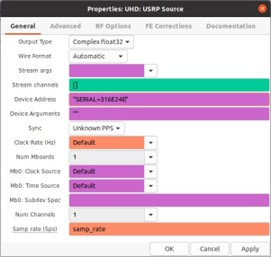
\includegraphics[width=.5\textwidth]{grc_success.jpg}
                \caption{}
                \label{fig:grcSucc}
            \end{figure}
        
        \section*{\textsf{Αντιμετώπιση Προβλημάτων}}
            Εάν για οποιονδήποτε λόγο αποτύχει η εγκατάσταση του προγράμματος οδήγησης UHD, 
            μπορείτε πάντα να εγκαταστήσετε το πρόγραμμα οδήγησης με μη αυτόματο τρόπο. 
            Μεταβείτε στο (εικόνες UHD)  και εξαγάγετε το ληφθέν αρχείο zip.
        
            \begin{lstlisting}[language=bash]
                $ uhd-images_*-release/share/uhd/
                $ cp -r images/ /usr/share/uhd
            \end{lstlisting}

\end{document}